\documentclass{article}
\usepackage[UTF8]{ctex}
% Replace `letterpaper' with`a4paper' for UK/EU standard size
\usepackage[a4paper,top=2cm,bottom=2cm,left=3cm,right=3cm,marginparwidth=1.75cm]{geometry}

% Useful packages
\usepackage{amsmath}
\usepackage{mathrsfs,amsmath}
\usepackage{graphicx}
\usepackage[colorlinks=true, allcolors=blue]{hyperref}
\usepackage{graphicx} %插入图片的宏包
\usepackage{float} %设置图片浮动位置的宏包
\usepackage{subfigure} %插入多图时用子图显示的宏包
\usepackage{parskip}
\usepackage{indentfirst} 
\setlength{\parindent}{2em}
\usepackage{hyperref}  
\usepackage{tikz}
\allowdisplaybreaks
\usepackage{multirow}
\usepackage{amsmath}
\usepackage{amsfonts,amssymb} 
\usepackage{xcolor} % 用于显示颜色
\usepackage{listings} % 用于插入代码
\lstset{
	basicstyle          =   \sffamily,          % 基本代码风格
	keywordstyle        =   \bfseries,          % 关键字风格
	commentstyle        =   \rmfamily\itshape,  % 注释的风格,斜体
	stringstyle         =   \ttfamily,  % 字符串风格
	flexiblecolumns,                % 别问为什么,加上这个
	numbers             =   left,   % 行号的位置在左边
	showspaces          =   false,  % 是否显示空格,显示了有点乱,所以不现实了
	numberstyle         =   \zihao{-5}\ttfamily,    % 行号的样式,小五号,tt等宽字体
	showstringspaces    =   false,
	captionpos          =   t,      % 这段代码的名字所呈现的位置,t指的是top上面
	frame               =   lrtb,   % 显示边框
}

\lstdefinestyle{Python}{
	language        =   Python, % 语言选Python
	basicstyle      =   \zihao{-5}\ttfamily,
	numberstyle     =   \zihao{-5}\ttfamily,
	keywordstyle    =   \color{blue},
	keywordstyle    =   [2] \color{teal},
	stringstyle     =   \color{magenta},
	commentstyle    =   \color{red}\ttfamily,
	breaklines      =   true,   % 自动换行,建议不要写太长的行
	columns         =   fixed,  % 如果不加这一句,字间距就不固定,很丑,必须加
	basewidth       =   0.5em,
}

\title{图像处理与可视化Homework-5 报告}
\author{林子开 21307110161}
\begin{document}
	\maketitle
	\tableofcontents

\section{主要Python文件简介}
由于实现本次作业的代码文件比较复杂,下面进行简要说明。
\begin{itemize}
    \item \texttt{white$\_$noise$\_$generator.py}文件能够生成白噪声。白噪声的频谱为1,相位角服从均匀分布或正态分布,允许用户从中选择。
    \item  \texttt{Rayleigh$\_$noise$\_$generator.py}文件能够生成瑞利噪声。
    \item \texttt{1$\_$adding$\_$noise.py}文件向测试用图分别添加不同强度白噪声或瑞利噪声。
    \item \texttt{2$\_$best$\_$notch$\_$filter.py}文件实现了最佳陷波滤波器,以上次作业带斜纹的噪声的脑膜图为测试用图。
\end{itemize}

\section{噪声的生成}

\subsection{白噪声的生成}
\paragraph{噪声原理介绍}
在\texttt{white$\_$noise$\_$generator.py}文件中,函数\texttt{generator$\_$w}实现了白噪声的生成。
在该函数中,白噪声的\textbf{频谱均取常数$1$};相位角有两种选择:
(1)服从$[0,2\pi]$上的均匀分布,(2)服从$\mathcal{N}(0,\pi)$的正态分布。
对频域进行傅里叶逆变换后,对时域取实部,并且进行归一化:$\tilde{n}(i,j) = n(i,j)/n_{max}$,
其中$n_{max} = \mathop{max}_{i,j}\,|n(i,j)|$。  

\paragraph{白噪声生成代码}
生成白噪声的Python代码如下:
\lstinputlisting[style = Python,
caption={Python codes to generate white noise}]{white_noise_generator.py} 


\subsection{瑞利噪声的生成}
\paragraph{噪声原理介绍}
在\texttt{Rayleigh$\_$noise$\_$generator.py}文件中,函数\texttt{generator$\_$r}实现了瑞利噪声的生成。
该函数产生服从分布$p(z)=\frac{2}{b}(z-a)\exp\left\{-\frac{(z-a)^2}{b}\right\},\,z\ge a$的瑞利噪声。
与产生白噪声的函数类似,产生瑞利噪声函数在返回噪声时也会进行归一化:$\tilde{n}(i,j) = n(i,j)/n_{max}$,
其中$n_{max} = \mathop{max}_{i,j}\,|n(i,j)|$。

\paragraph{瑞利噪声生成代码}
生成瑞利噪声的Python代码如下:
\lstinputlisting[style = Python,
caption={Python codes to generate Rayleigh noise}]{Rayleigh_noise_generator.py} 

\subsection{向测试图像添加噪声}
\paragraph{添加噪声的细节说明}
添加噪声的数学公式为
\[
\hat{f}(x,y) = f(x,y) + c\eta(x,y)    
\]

其中,$\eta(x,y)$分别选取相位角服从均匀分布的白噪声,相位角服从正态分布的白噪声,以及瑞利噪声。
三类噪声均提前进行了归一化处理。系数$c$则代表了\textbf{噪声强度},在本次实验中,分别取$c=50,100,150$。
在添加噪声后,对于超出$[0,255]$区间的灰度值,统一进行截断处理。

\paragraph{添加噪声的代码实现}
向图像中添加噪声的Python代码如下:
\lstinputlisting[style = Python,
caption={Python codes to add noise}]{1_adding_noise.py} 

\paragraph{添加噪声后的效果}
以下是对大脑图像添加不同类型、不同强度噪声后的效果

\begin{figure}[H]
    \centering
    \subfigure[c=50]
    { 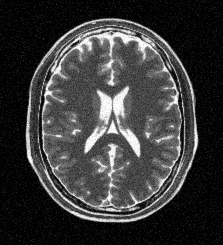
\includegraphics[width=0.3\textwidth]{adding_noise_result//大脑图像 c=50 uniform white noise.png}}
    \,    
    \subfigure[c=100]
    { 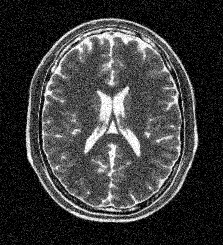
\includegraphics[width=0.3\textwidth]{adding_noise_result//大脑图像 c=100 uniform white noise.png}}
    \,
    \subfigure[c=150]
    { 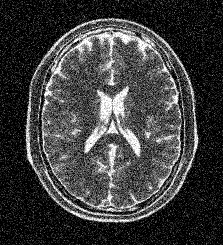
\includegraphics[width=0.3\textwidth]{adding_noise_result//大脑图像 c=150 uniform white noise.png}}
    \caption{向大脑图像添加相位角服从均匀分布的白噪声} 
\end{figure}


\begin{figure}[H]
    \centering
    \subfigure[c=50]
    { 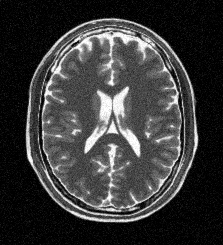
\includegraphics[width=0.31\textwidth]{adding_noise_result//大脑图像 c=50 Gauss white noise.png}}
    \,    
    \subfigure[c=100]
    { 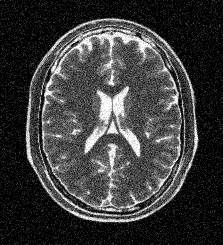
\includegraphics[width=0.31\textwidth]{adding_noise_result//大脑图像 c=100 Gauss white noise.png}}
    \,
    \subfigure[c=150]
    { 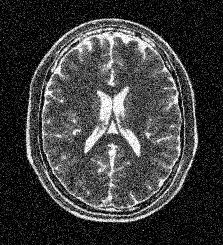
\includegraphics[width=0.31\textwidth]{adding_noise_result//大脑图像 c=150 Gauss white noise.png}}
    \caption{向大脑图像添加相位角服从$\mathcal{N}(0,\pi)$正态分布的白噪声} 
\end{figure}


\begin{figure}[H]
    \centering
    \subfigure[c=50]
    { 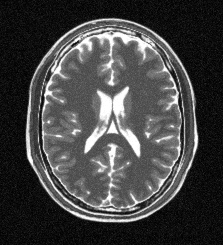
\includegraphics[width=0.31\textwidth]{adding_noise_result//大脑图像 c=50 Rayleigh noise.png}}
    \,    
    \subfigure[c=100]
    { 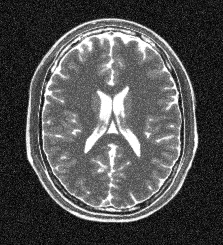
\includegraphics[width=0.31\textwidth]{adding_noise_result//大脑图像 c=100 Rayleigh noise.png}}
    \,
    \subfigure[c=150]
    { 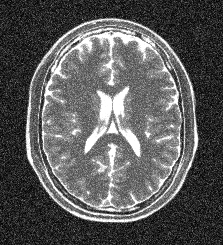
\includegraphics[width=0.31\textwidth]{adding_noise_result//大脑图像 c=150 Rayleigh noise.png}}
    \caption{向大脑图像添加瑞利噪声} 
\end{figure}

以下是对心脏图像添加不同类型、不同强度噪声后的效果

\begin{figure}[H]
    \centering
    \subfigure[c=50]
    { 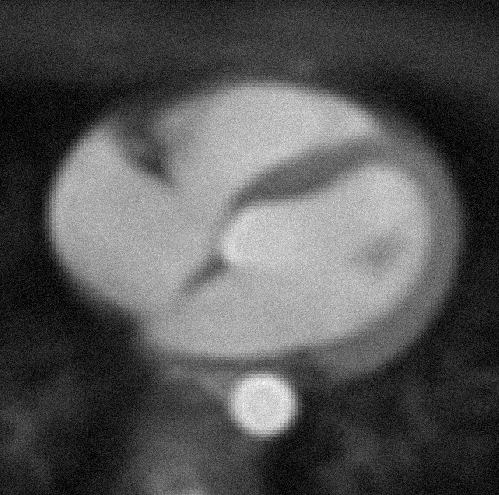
\includegraphics[width=0.31\textwidth]{adding_noise_result//心脏图像 c=50 uniform white noise.png}}
    \,    
    \subfigure[c=100]
    { 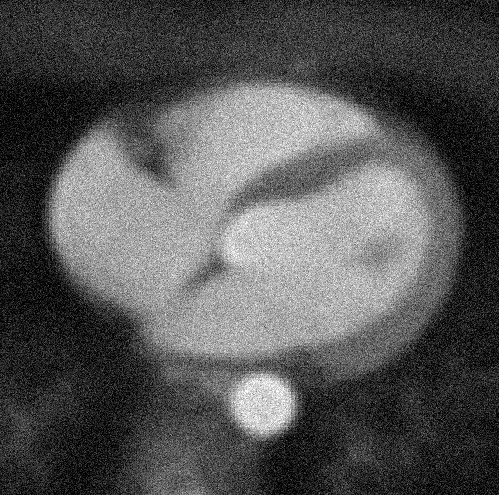
\includegraphics[width=0.31\textwidth]{adding_noise_result//心脏图像 c=100 uniform white noise.png}}
    \,
    \subfigure[c=150]
    { 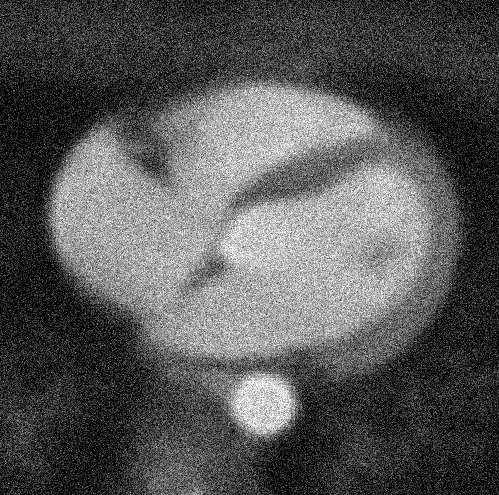
\includegraphics[width=0.31\textwidth]{adding_noise_result//心脏图像 c=150 uniform white noise.png}}
    \caption{向心脏图像添加相位角服从均匀分布的白噪声} 
\end{figure}


\begin{figure}[H]
    \centering
    \subfigure[c=50]
    { 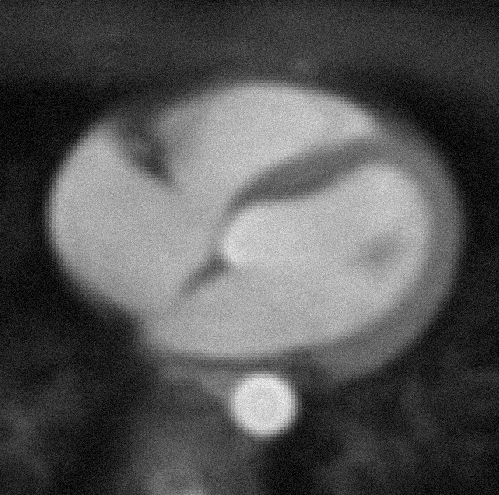
\includegraphics[width=0.31\textwidth]{adding_noise_result//心脏图像 c=50 Gauss white noise.png}}
    \,    
    \subfigure[c=100]
    { 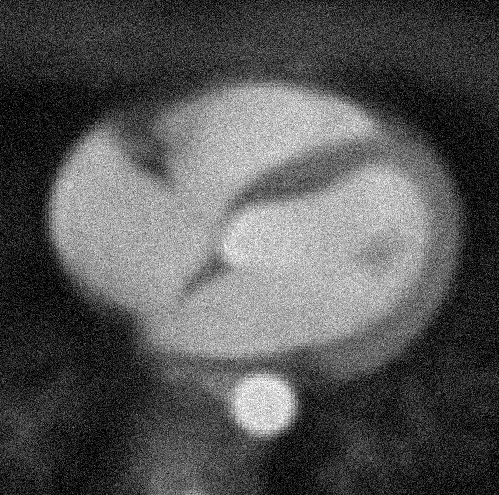
\includegraphics[width=0.31\textwidth]{adding_noise_result//心脏图像 c=100 Gauss white noise.png}}
    \,
    \subfigure[c=150]
    { 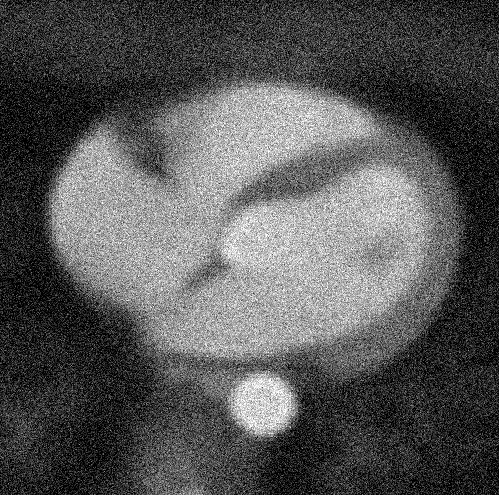
\includegraphics[width=0.31\textwidth]{adding_noise_result//心脏图像 c=150 Gauss white noise.png}}
    \caption{向心脏图像添加相位角服从$\mathcal{N}(0,\pi)$正态分布的白噪声} 
\end{figure}


\begin{figure}[H]
    \centering
    \subfigure[c=50]
    { 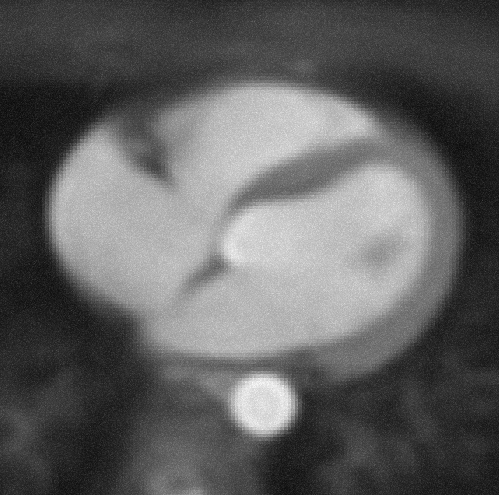
\includegraphics[width=0.31\textwidth]{adding_noise_result//心脏图像 c=50 Rayleigh noise.png}}
    \,    
    \subfigure[c=100]
    { 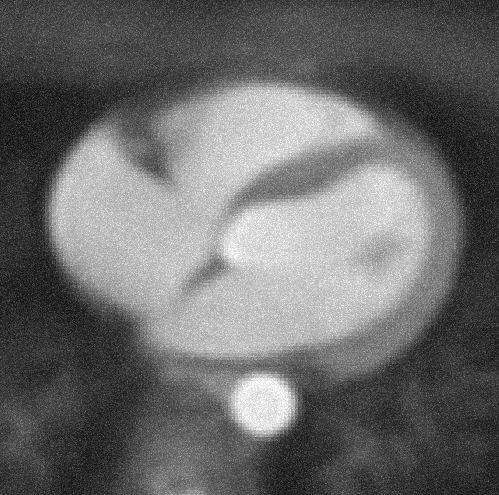
\includegraphics[width=0.31\textwidth]{adding_noise_result//心脏图像 c=100 Rayleigh noise.png}}
    \,
    \subfigure[c=150]
    { 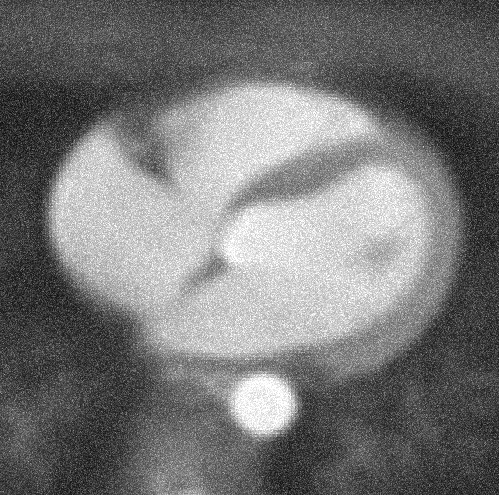
\includegraphics[width=0.31\textwidth]{adding_noise_result//心脏图像 c=150 Rayleigh noise.png}}
    \caption{向心脏图像添加瑞利噪声} 
\end{figure}

\section{最佳陷波滤波器}
\subsection{最佳陷波滤波器的原理}
首先观察带噪声图像的频域图像,构建频域滤波器,得到噪声的频域函数$N(u,v)$。
对$N(u,v)$进行傅里叶逆变换,得到噪声的时域函数$\eta(x,y)=\mathscr{F}^{-1}\{N(u,v)\}$。

进行时域滤波时,需要对含噪声的图像进行如下去噪操作:
\[
\hat{f}(x,y) = g(x,y) - w(x,y)\eta(x,y)	
\]
其中$w(x,y)$为调制函数,表达式可以简写为:
\[
w(x,y) = \frac{\overline{g\eta}-\bar{g}\bar{\eta}}{\bar{\eta^2}-\bar{\eta}^2}	
\]
$g(x,y)$和$\eta(x,y)$分别是以$(x,y)$为中心的邻域上的原图灰度值和噪声灰度值。
不同的邻域大小可能产生不同的$w(x,y)$。

\subsection{Python代码实现}
实现最佳陷波滤波器的Python代码如下所示。
\lstinputlisting[style = Python,
caption={Python codes of optimal notch filter}]{2_best_notch_filter.py} 

\subsection{滤波效果展示}
选取Homework-4所提供的带噪声的脑膜图作为测试图,如图\ref{test}所示。
\begin{figure}[H]
	\centering
	{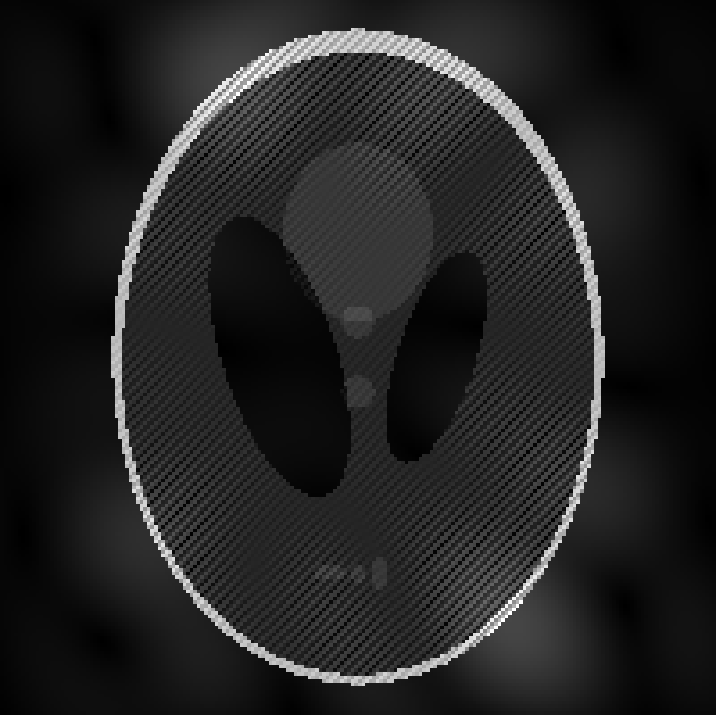
\includegraphics[width=0.35\textwidth]{带噪声的脑膜图.PNG}} 
	\caption{测试用途:带噪声的脑膜图}   \label{test}
\end{figure}


首先根据频谱,构建相应的频域滤波器,提取噪声的频域函数。
原图的频谱如图\ref{fig1.sub.1}所示。根据原图频谱,构建相应的频域滤波器,如图\ref{fig1.sub.2}所示。
\begin{figure}[H]
    \centering
    \subfigure[原图频谱]
    { \label{fig1.sub.1} 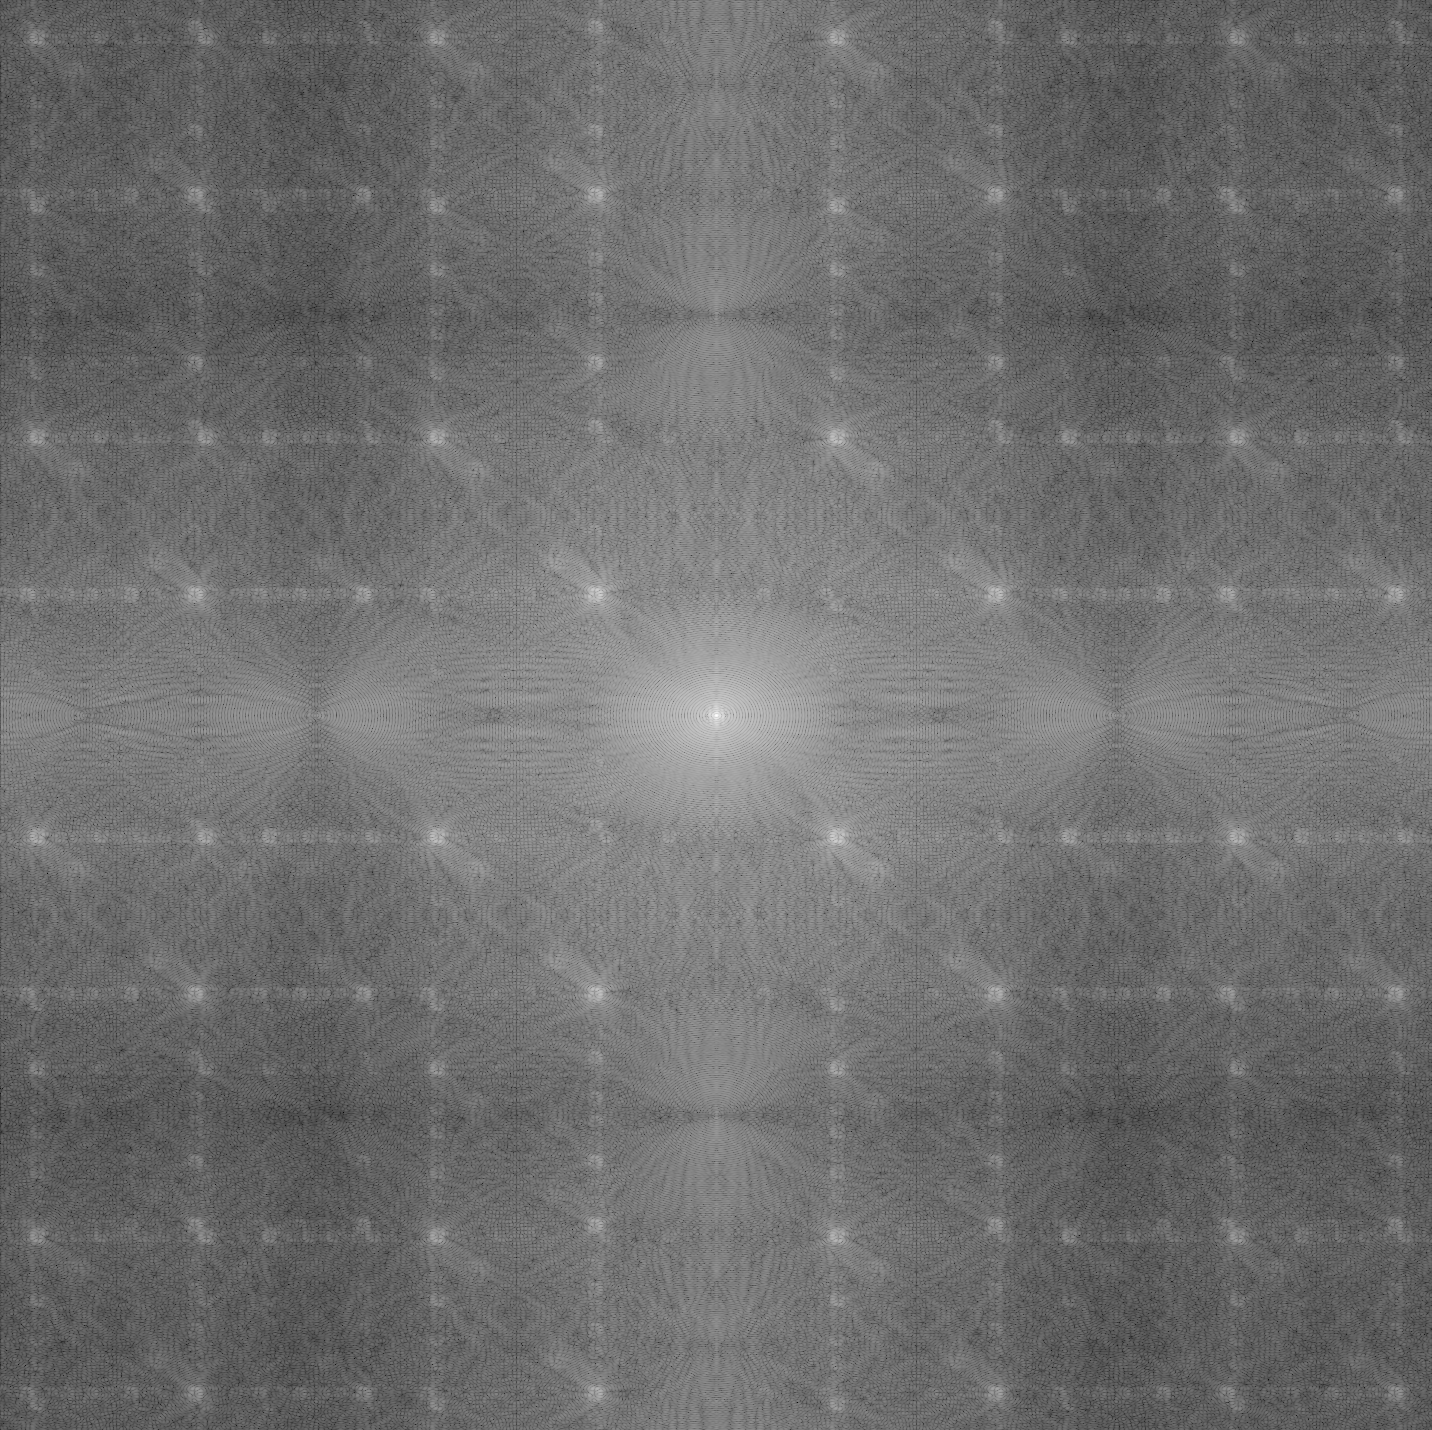
\includegraphics[width=0.35\textwidth]{notch_filter_result//原图的频谱.png}}
    \,    
    \subfigure[噪声的频域滤波器]
    { \label{fig1.sub.2} 
\includegraphics[width=0.35\textwidth]{notch_filter_result//噪声滤波器示意图.png}}
    \caption{原图频谱和噪声的频域滤波器}  \label{fig1.main}
\end{figure}


用该频域滤波器对原图频谱进行频域滤波,得到噪声的频域函数$N(u,v)$,如图\ref{fig2.sub.1}所示。
由噪声的频域图像,得到噪声的时域函数$\eta(x,y)$,如图\ref{fig2.sub.2}所示。
\begin{figure}[H]
    \centering
    \subfigure[噪声的频域图像]
    { \label{fig2.sub.1} 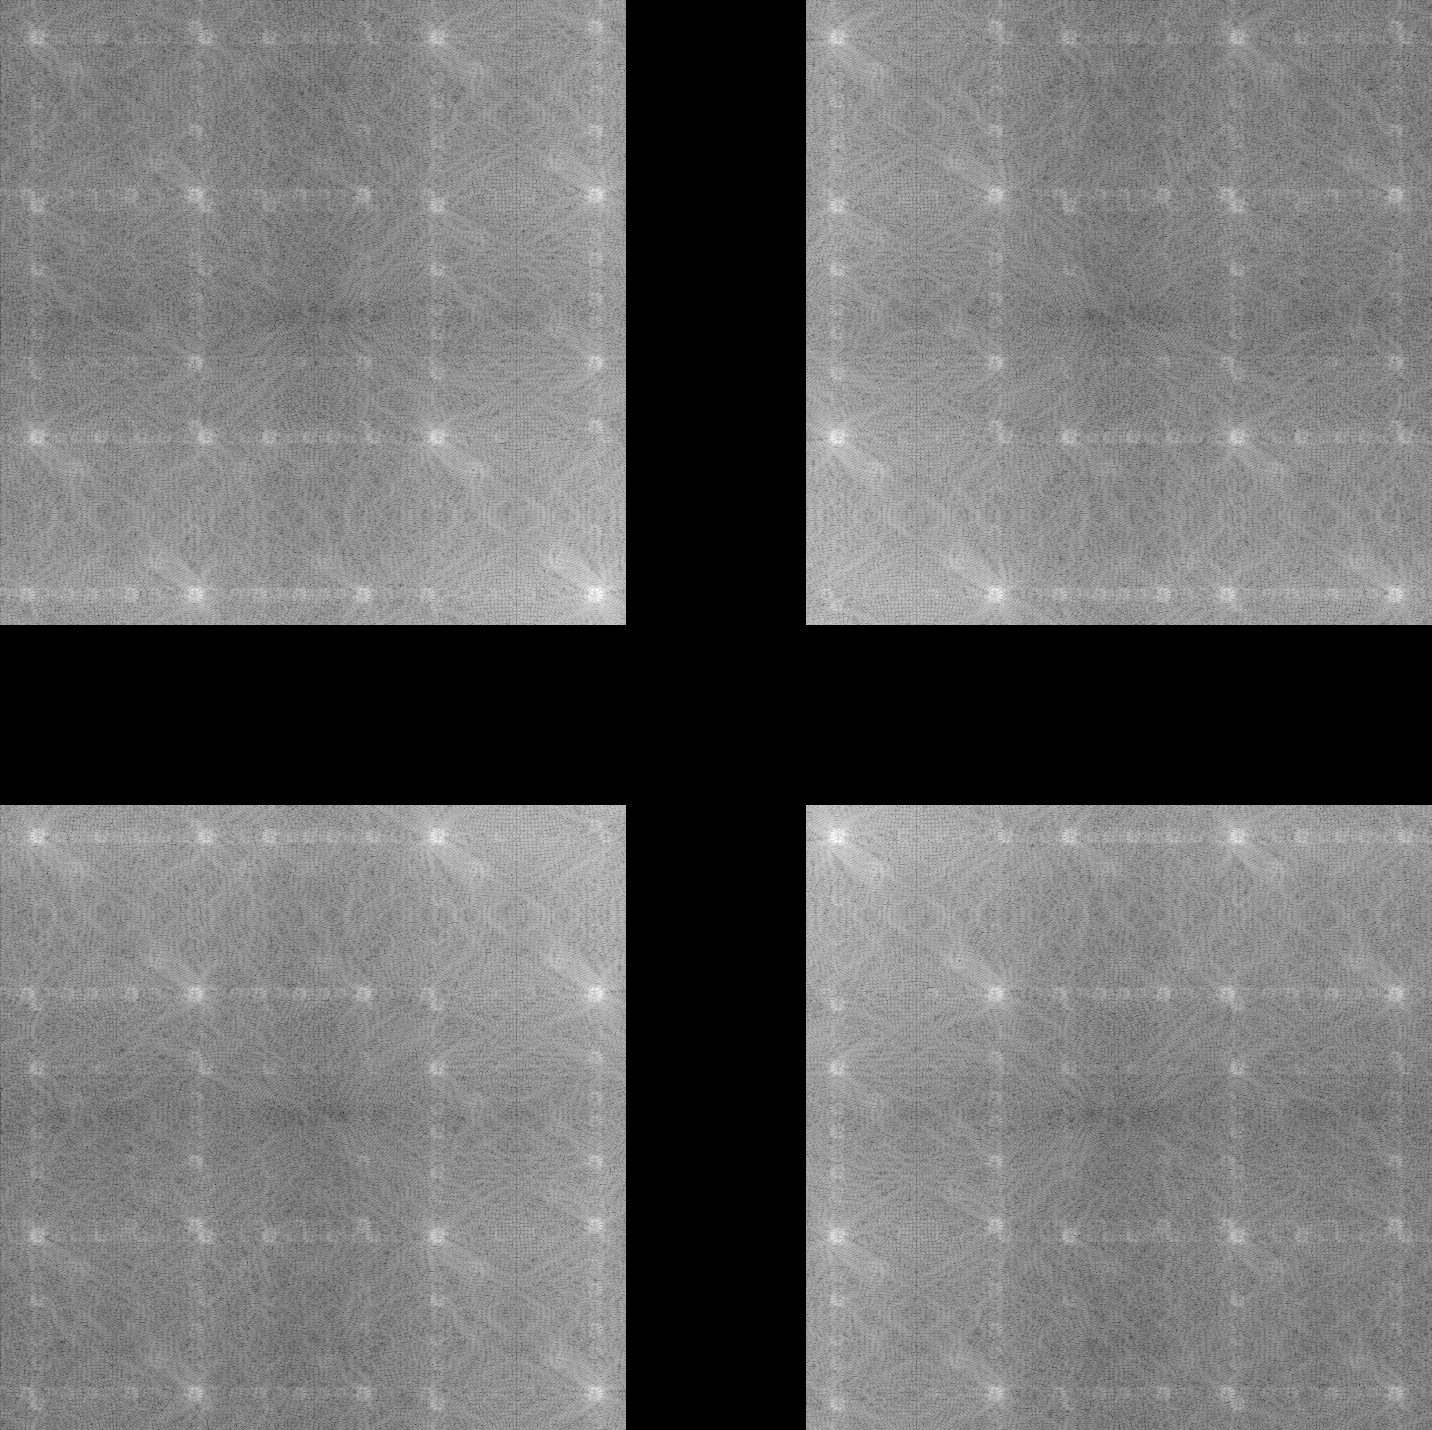
\includegraphics[width=0.45\textwidth]{notch_filter_result//噪声的频域图像.png}}
    \,    
    \subfigure[噪声的时域图像]
    { \label{fig2.sub.2} 
\includegraphics[width=0.45\textwidth]{notch_filter_result//噪声图像.png}}
    \caption{噪声的频域和时域图像}  \label{fig2.main}
\end{figure}

尝试不同的邻域大小(要求为奇数)的滤波效果如下:
\begin{figure}[H]
    \centering
    \subfigure[patch size = 3]
    { 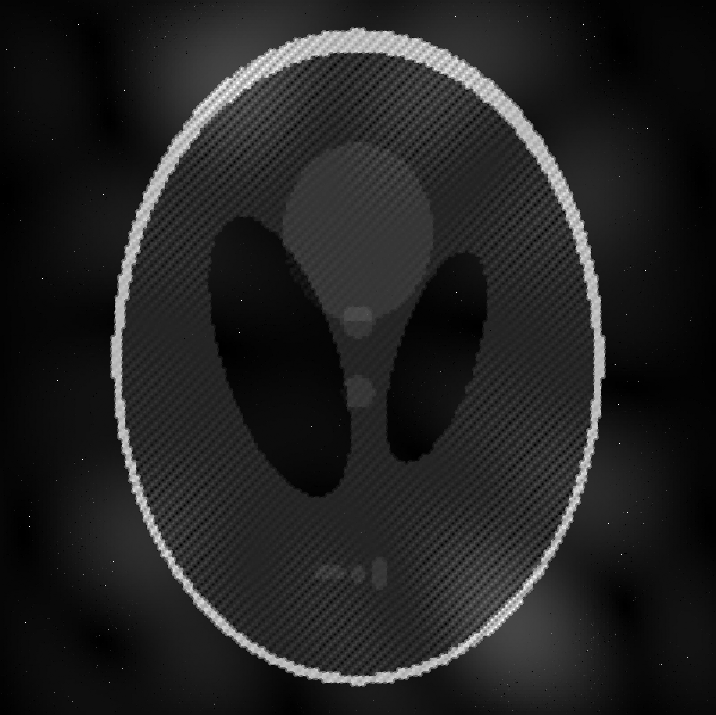
\includegraphics[width=0.3\textwidth]{notch_filter_result//滤波后的图像 patchSize=3.png}}
    \,    
	\subfigure[patch size = 5]
    { 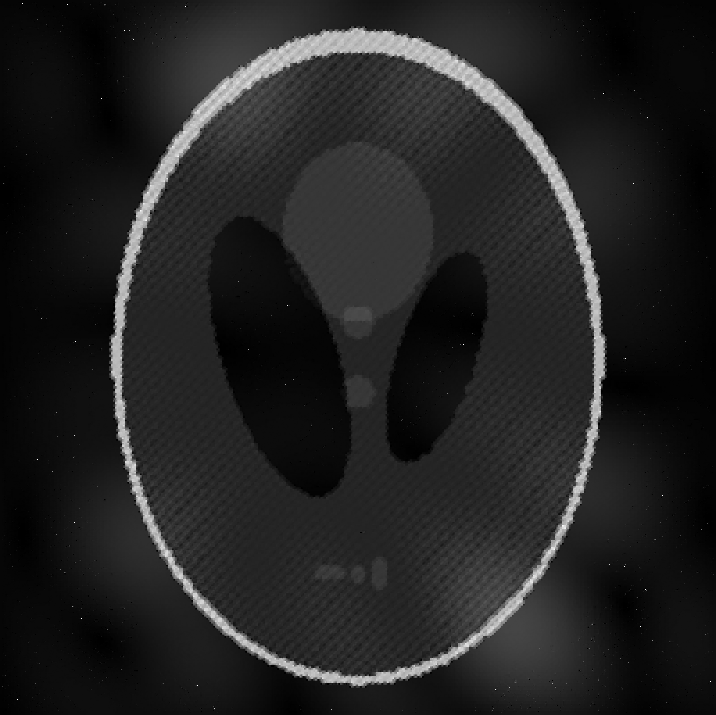
\includegraphics[width=0.3\textwidth]{notch_filter_result//滤波后的图像 patchSize=5.png}}
    \, 
	\subfigure[patch size = 7]
    { 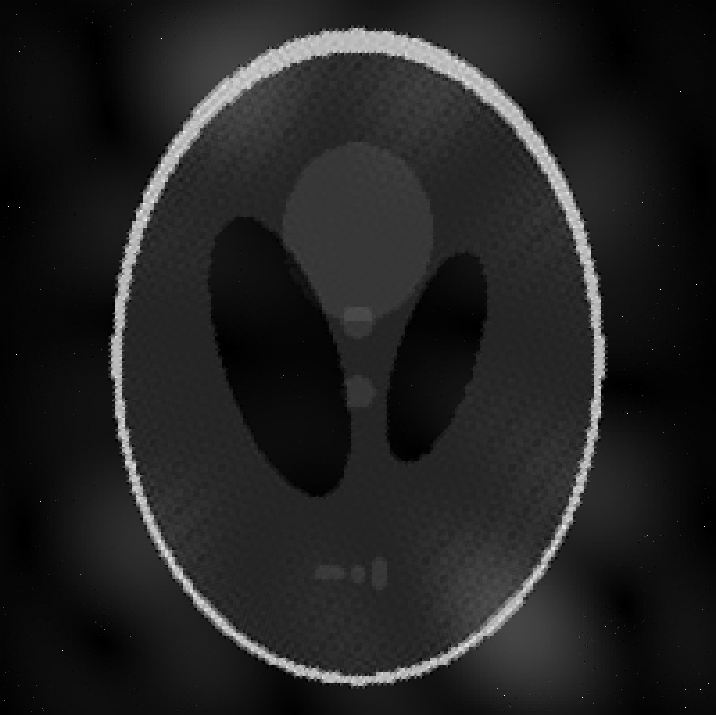
\includegraphics[width=0.3\textwidth]{notch_filter_result//滤波后的图像 patchSize=7.png}}
    \, 
	\subfigure[patch size = 9]
    { 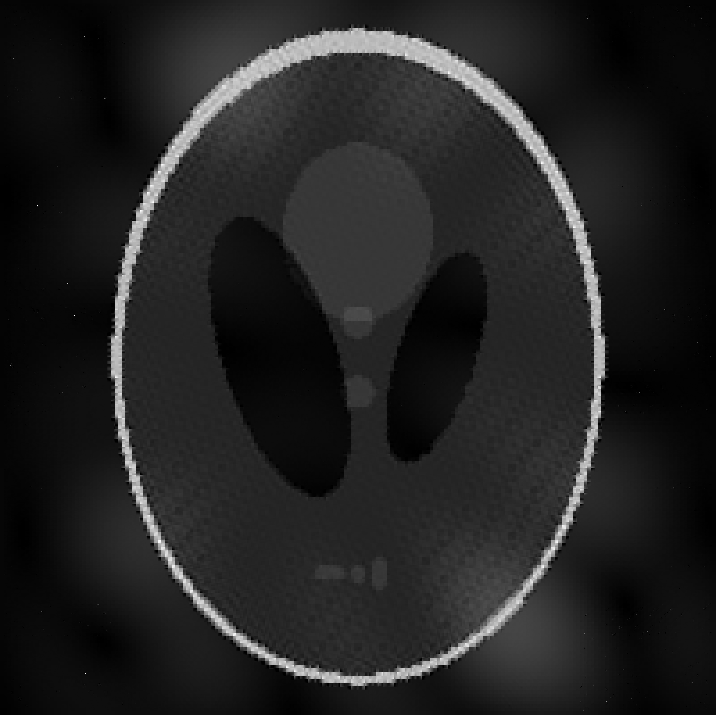
\includegraphics[width=0.3\textwidth]{notch_filter_result//滤波后的图像 patchSize=9.png}}
    \, 
	\subfigure[patch size = 11]
    { 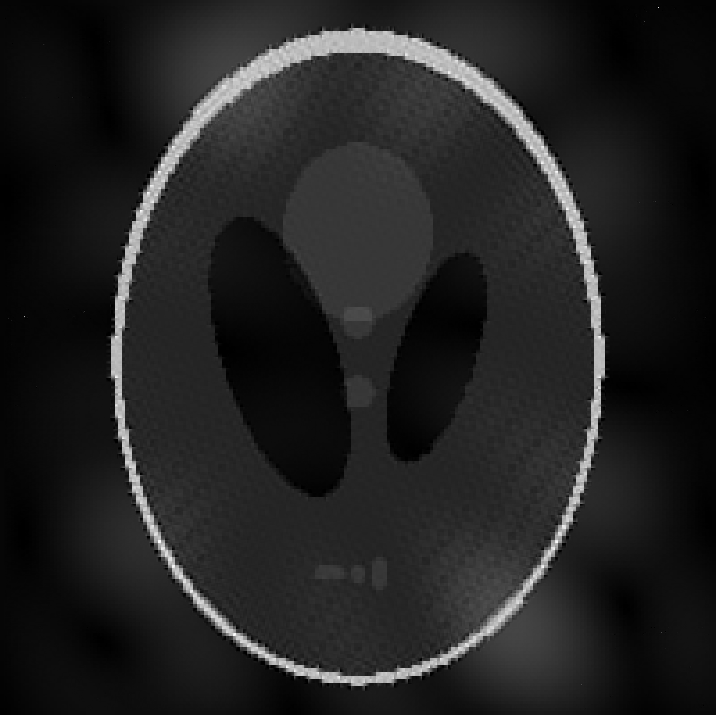
\includegraphics[width=0.3\textwidth]{notch_filter_result//滤波后的图像 patchSize=11.png}}
    \, 
	\subfigure[patch size = 13]
    { 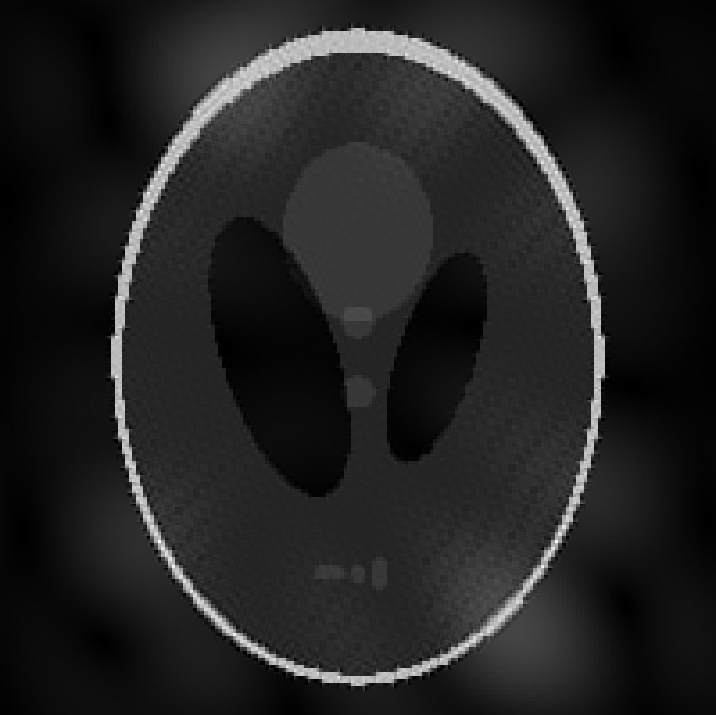
\includegraphics[width=0.3\textwidth]{notch_filter_result//滤波后的图像 patchSize=13.png}}
	\caption{基于不同邻域大小的最佳陷波滤波器的滤波效果} 
\end{figure}

可以看出,当邻域大小patchSize=7时,滤波效果已经比较好;当继续增加patchSize,滤波效果不再有显著改变。
因此,在本次实验中,对于该测试用图,邻域大小取7是比较合适的。

\end{document}

% \begin{figure}[H]
% 	\centering
% 	{\includegraphics[width=0.315\textwidth]{image//ignorance.png}} 
% 	\caption{}  
% \end{figure}


% \lstinputlisting[style = Python,
% caption={Python codes},
% label = {efficient},
% linerange={110-125}]{exercise3.py} 


% \begin{figure}[H]
%     \centering
%     \subfigure[patch size = 11]
%     { 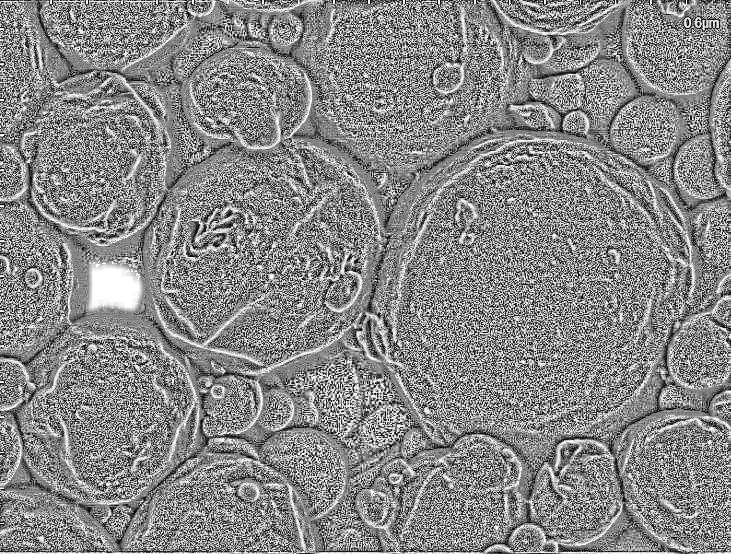
\includegraphics[width=0.45\textwidth]{image//local equalization with patch size = 11.jpg}}
%     \,    
%     \subfigure[patch size = 51]
%     { 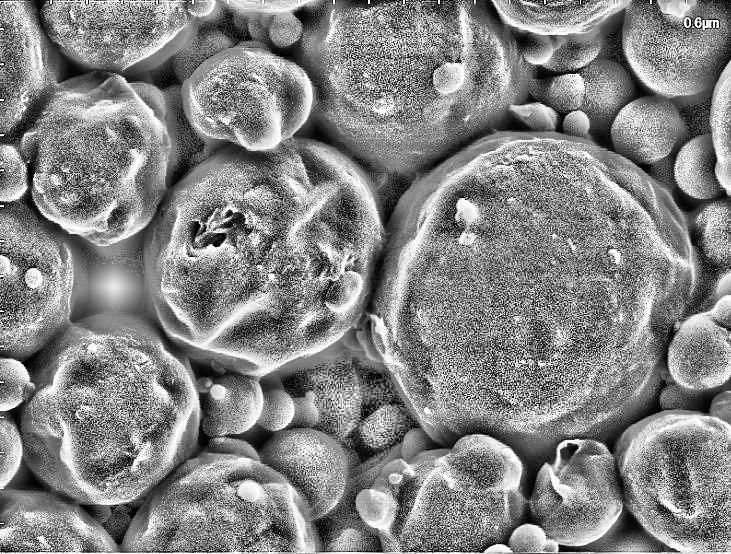
\includegraphics[width=0.45\textwidth]{image//local equalization with patch size = 51.jpg}}
%     \,
%     \subfigure[patch size = 151]
%     { 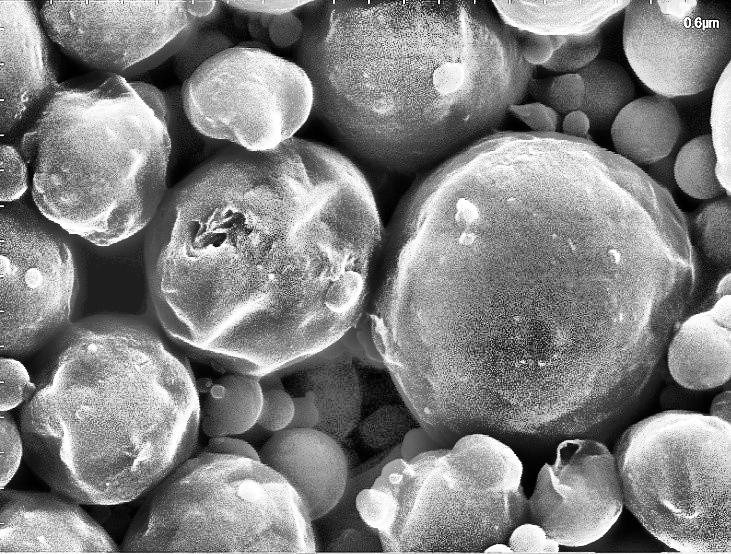
\includegraphics[width=0.45\textwidth]{image//local equalization with patch size = 151.jpg}}
%     \,    
%     \subfigure[patch size = 201]
%     { 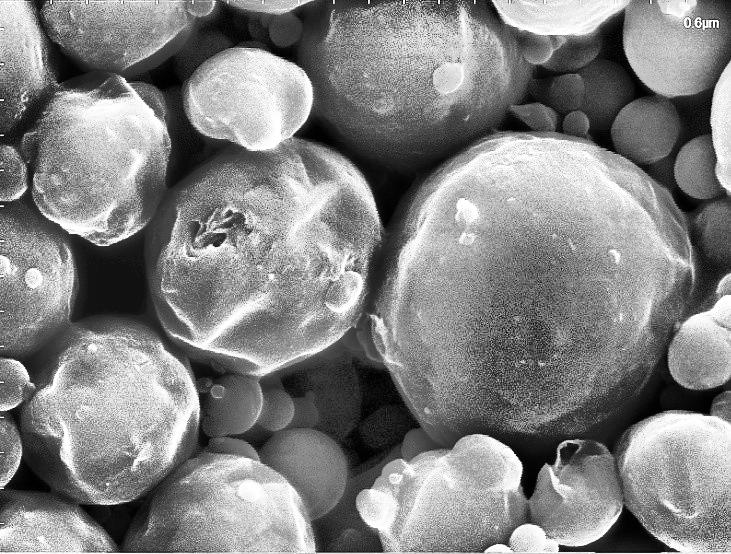
\includegraphics[width=0.45\textwidth]{image//local equalization with patch size = 201.jpg}}
%     \caption{local equalization with different patch sizes} 
% \end{figure}
